\documentclass[oneside,openany,11pt,a4paper,fontsize=11pt]{report}

\usepackage[utf8]{inputenc}

\usepackage[T1]{fontenc}
\usepackage{graphicx}
\usepackage{titlesec}
\usepackage[left=2.5cm,right=2.5cm,top=3cm,bottom=3cm]{geometry}


%nastavení fontů
\usepackage{sectsty}
\usepackage{fontspec}

%ToDo Zjistit, jestli to musí být tyto fonty
%\setmainfont{Cambria}
%\setsansfont{Calibri}
\setsansfont{Helvetica}

%bezpatkové nadpisy
\partfont{\normalfont\sffamily\bfseries}
\chapterfont{\normalfont\sffamily\bfseries}
\sectionfont{\normalfont\sffamily\bfseries}
\subsectionfont{\normalfont\sffamily\bfseries}

%Vyhození názvu kapitoly
\titleformat{\chapter}{\sffamily\huge}{\thechapter.}{20pt}{\huge}

%řádkování
\usepackage{setspace}
\renewcommand{\baselinestretch}{1.5}

% zarovnání nadpisu abstraktu doleva
\usepackage{abstract}
\renewcommand{\absnamepos}{flushleft}
\setlength{\absleftindent}{0pt}
\setlength{\absrightindent}{0pt}
% abstrakt bezpatkovým písmem
\renewcommand{\abstractnamefont}{\sffamily\large\bfseries}
% zrušení vertikálního centrování stránky abstraktu
\usepackage{etoolbox}
\patchcmd{\abstract}{\null\vfil}{}{}{}

%odsazení paragrafů prázdným řádkem
\usepackage[parfill]{parskip}

%command pro novou prázdnou stránku
\usepackage{afterpage}

%vytvoření příkazu pro prázdnou stránky
\newcommand\blankpage{%
    \null
    \thispagestyle{empty}%
    \addtocounter{page}{-1}%
    \newpage}
    
%vytvoření příkazu pro podpisovou linku
\newcommand*{\SignatureAndDate}[1]{    
    \par\noindent\makebox[2.5in][l]{In \makebox[1.0in]{\dotfill} on \makebox[1.0in]{\dotfill}} \hfill\makebox[2.0in]{\dotfill}
    \par\noindent\makebox[2.5in]{~}      \hfill\makebox[2.0in]{#1}
    

}
%sloupce
\usepackage{multicol}

%obrázky
\usepackage{tikz}
\usepackage{geometry}

%odkazy
\usepackage{hyperref}

%ToDo Harvardské citace
%\usepackage{natbib}
%\setcitestyle{round}

%vícestránkové tabulky
\usepackage{longtable}

\usepackage{float}

\usepackage[toc,page]{appendix}

%přejmenování seznamů
\renewcommand{\listfigurename}{List of images}
\renewcommand{\listtablename}{List of tables}


\begin{document}

%vypnout číslování, zapínáme až na první číslované stránce
\pagenumbering{gobble}

%Úvodní stránka
\begin{minipage}[t]{\textwidth}
	\centering
	\sffamily{\Large{\uppercase{Unicorn College}}}
\end{minipage}


\vspace*{\fill}
	\begin{center}
		\sffamily{\Huge{\uppercase{Bakalářská práce}}}
	\end{center}
\vspace*{\fill}


\begin{minipage}[b]{\textwidth}

\begin{minipage}[b]{0.5\linewidth}
	\sffamily{\Large{\the\year}}
\end{minipage}
\quad
\begin{minipage}[b]{0.5\linewidth}
	\begin{flushright}
		\sffamily{\Large{Josef SEKAVA}}
	\end{flushright}
\end{minipage}
\end{minipage}

%Stránka s erbem školy
\newpage
\begin{figure}[t]
	\centering
	\sffamily{\Large{\uppercase{Unicorn College}}} \\
	\vspace{\baselineskip}
	\sffamily{\large{Department of Information Technologies}}
\end{figure}



\vspace*{\fill}
	\begin{figure}[h]
		\centering
		
\includegraphics[width=0.5\textwidth]{img/UCL_erb.png}\\
		\sffamily{\Large{\uppercase{Bakalářská práce}}} \\
		\vspace{\baselineskip}
		\sffamily{\large{The Web Service API layer for the Component Database for ATLAS Inner Detector~at~LHC}}
	\end{figure}
\vspace*{\fill}





\begin{figure}[b]


		\sffamily{\textbf{Autor~BP:} Josef~Sekava}\\
		\sffamily{\textbf{Vedoucí~BP:} Ing.~Marek~Beránek,~Ph.D.} \\

\vspace{\baselineskip}
\vspace{\baselineskip}
	
	\begin{minipage}[b]{0.5\linewidth}
		\sffamily{\the\year}
	\end{minipage}
	\quad
	\begin{minipage}[b]{0.5\linewidth}
		\begin{flushright}
			\sffamily{Praha}
		\end{flushright}
	\end{minipage}
\end{figure}


%Prázdná stránka
\afterpage{\blankpage}

%Deklarace
\newpage
\null
\vfill
\section*{Declaration}
I thereby declare, that I have written my bachelor thesis on topic \emph{The Web Service API layer for the Component Database for ATLAS Inner Detector at LHC} independently under the supervision of the advisor of my bachelor thesis and using exclusively those external sources, directly or indirectly, that are listed in the Bibliography section of this thesis.

As an author of this bachelor thesis I declare that did not violate any copyright of any third parties and that I am fully aware of the consequences of violating the provisions §~11 and those following in the law \emph{on Copyright and Rights Related to Copyright and on Amendment to Certain Acts} no.~121/2000~Coll.

\vspace{\baselineskip}

	\SignatureAndDate{(Josef Sekava)}



%ToDo Poděkování
\newpage
\null
\vfill
\section*{Acknowledgements} Lorem ipsum dolor sit amet, consectetur adipiscing elit. Mauris id congue neque. Nullam porta vestibulum diam, non dictum turpis hendrerit aliquet. Vivamus ac turpis nec ligula vulputate sollicitudin eget ut velit. Nunc eu gravida justo. Fusce et pharetra sapien. Morbi dui ante, interdum eu pretium sed, finibus et purus. Pellentesque quis dolor dui. Interdum et malesuada fames ac ante ipsum primis in faucibus. Curabitur ultrices posuere nibh, at auctor nunc finibus ac. Mauris facilisis interdum mauris eu suscipit. Ut ultricies porta libero, in scelerisque odio viverra et. Fusce felis ligula, aliquet at lorem at, pharetra egestas purus. Aenean gravida, neque quis sodales sagittis, justo purus tristique velit, in pharetra massa elit at ipsum. Nullam porttitor tortor augue, eget auctor neque fringilla ac.



%První číslovaná strana
\newpage

%zde zapínáme znovu číslování stránek
\setcounter{page}{1}
\pagenumbering{arabic}

\tikz[remember picture,overlay] \node[opacity=1.0,inner sep=0pt] at (current page.center){
\includegraphics[width=\paperwidth,height=\paperheight]{img/prvni_cislovana_strana.jpg}};



\vspace*{\stretch{2}}
\begin{center}
\begin{minipage}{.6\textwidth}
	\begin{center}
	\sffamily{\large
	{The Web Service API layer for the Component Database for ATLAS Inner Detector~at~LHC}}
	\end{center}
\end{minipage}
\end{center}
\vspace{\stretch{3}}
\clearpage

\newpage

\begin{abstract}
\setcounter{page}{2}
\thispagestyle{plain} 
\par At present, the Component Database for ATLAS Inner Detector at LHC is still in development and it’s missing several important parts and features. The goal of this bachelor thesis is to gather and analyse the requirements for the Production database for the ATLAS experiment Inner Tracker, propose the architecture and implement the API layer that meets the required demands.

\paragraph{The second part} of this thesis is dedicated to gathering of the data required to understand the problematic of the ATLAS experiment and cooperating institutions.

\paragraph{The third part} of the application describes the requirements for the API layer, based on the research

\paragraph{The fourth part} proposes the architecture of the API layer shows mockups for the example resources and describes the inner functionality of the API application.

\par Considering the nature of the database content, special care is given to the authorisation and user authentication to protect the data in the database.

\paragraph{The fifth part} of this thesis is the implementation of the functional, usable and deployable REST API layer for the database.

\paragraph{The sixth part} describes the automated test that should assure the functionality of the database even when its functionality is extended in the future.

\paragraph{The seventh part} is the implementation of the simple web interface, which would use the API to provide access to stored data.

\paragraph{Keywords:} CERN, LHC, ATLAS, ITk, SCT, Component database, Production database, API, REST

\end{abstract}

\pagebreak

%table of contents
\setcounter{page}{3}
\tableofcontents
\pagebreak

%Thesis here
%Úvod (nečíslovaná kapitola)
\chapter{Introduction}
\label{chap:introduction}
\par The goal of this thesis is to gather and analyse the requirements for the Production database for the Inner Tracker upgrade project and in the next step, based on the findings, to propose and implement the standalone API Web Service application that is meeting the required demands with an example endpoint to demonstrate its functionality. The API application should be functional, usable and deployable.

\par The purpose of the API is to enable fast and easy access to the database data for users and also the 3rd party applications. The content of the thesis includes the process of gathering of necessary materials for a proper development and selection of the API type for data of the ITk database.

\par It results in relevant selection of programming languages and technologies (on premise and cloud services) for the implementation. A special is given to the matter of authorisation and user privileges handling. The full list and descriptions of proposed endpoints and their mockups is included as a part of the design proposal and the implementation of API application is demonstrated with the selected API endpoint.
\chapter{ITk upgrade}
\label{chap:itkUpgrade}

\par The following part is the introduction to the problematics of ITk layout and documents the current status of the component database.

\section{The Inner Tracker overview}
\par The ATLAS\footnote{\textbf{A} \textbf{T}oroidal \textbf{L}HC \textbf{A}pparatu\textbf{S}} experiment is one of the two general purpose experiments (the other being CMS) installed on the Large Hadron Collider (LHC) at the European Organization for Nuclear Research (CERN). Inside the LHC, bunches of 10\textsuperscript{11} protons will collide 40 million times per second.\cite[page 10]{atlasExperiment}


\par The ATLAS experiment is installed around the cross-section point\cite[page 10]{atlasExperiment} where the protons, after being accelerated on the LHC, collides in the measured collisions, which are tracked using the detectors on the experiment. 

\par The ATLAS is ~45 meters long and more than 25 meters high, and weighs about 7 000 tons. \cite{atlasweb}. The Inner detector (or inner tracker) is a cylindrical device 5 meters long with 2.3 meters in diameter \cite[page 10]{atlasExperiment} located in the very centre of the detector. It contains a large number of the high-resolution detectors of two main types: pixel and strips, which are positioned in several layers to maximise the measured area. The inner detector is the part of the experiment that is closest to the point of collision and measures the momentum of each charged particle. \cite{atlasitkweb}


\begin{figure}[!ht]
	\centering
	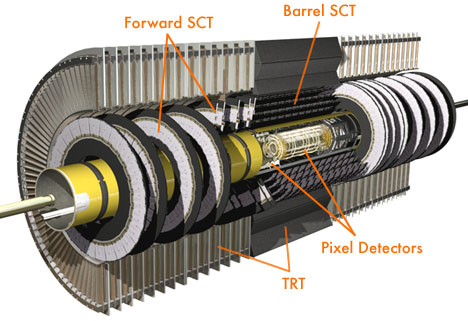
\includegraphics[width=0.6\textwidth]{img/itk_schema.jpg}\\	
	\caption{A schema of the ATLAS Inner tracker \cite{atlasitkweb}}
\end{figure}

\par The difference between the two main types of detectors, strips and pixels, is in their construction, purpose and location on the ITk central solenoid. The pixel detectors are " the high-precision detector layers, which are arranged on concentric cylinders around the beam axis, while the end-cap detectors (strips) are mounted on disks perpendicular to the beam axis".  \cite[page 14]{atlasExperiment}

\par For the purpose of this thesis, all the other parts of the detector, e.g. calorimeters, are opted out from this description, since both the current Component database and the proposed API layer does not include them in any of the use cases.

\section{The upgrade process}
\par The Inner tracker is scheduled for a replacement with the construction of the new detector beginning in the early 2017. The upgrade process involves the replacement of the entire detector with the newly designed detector that can measure collisions with much higher precision.

\par The new detector should be installed in 2018 and should be in operation until 2035. \cite{sverma}

\par Currently 94 academic institutions from 20 countries are cooperating in the effort to prepare and build the new Inner tracker. To synchronise the effort, centralise component database is being prepared to record and hold the following data: \cite[slide 4]{databasePresentation}

\begin{itemize}
	\item components used (mechanical, thermal, electrical, performance),
	\item performance for quality assurance process,
	\item details of construction of composite objects,
	\item physical location for logistical control,
	\item details of the production quality (mainly tests),
	\item any details for the future.
\end{itemize}

\par These requirements are more thoroughly explored in the following sections.

\section{Terminology}
\par The basic level of knowledge about the LHC, ATLAS experiment and ITk functionality is expected in this thesis. Some commonly used terms are described below:
\begin{description}
   \item[ITk] \hfil \\
		The Inner tracker (or the Inner detector) is the most inner part of the ATLAS experiment. It is used for the measuring of the momentum of each charged particle. \cite{atlasweb}
   \item[SCT database] \hfil \\
      	The database for the old inner detector
      	SCT (Semi-Conductor Tracker) is the middle section of the inner detector. \cite[17]{sverma} The SCT database is the original production database used by the last version of the ITk. Build on ORACLE 9i it was the primarily used database for the old ITk. \cite[25]{sverma} The usage statistics from it's production usage are listed in section~\ref{sec:databaseUsage}.
   \item[The Production database] \hfil \\
	The initial version of the Production database (Also "ITk database" or "Component database") was implemented in 2006 by Cambridge University as a next generation SCT database. \cite[p27]{sverma} It was designed for the purposes of the SCT and it lacks some advanced features required by institutions working on other parts of the inner tracker. The missing features are described more closely in the section~\ref{sec:notImplemented}.
	\item[Item] \hfil \\
	An Item is a general term for any component used when building the ITk structure. The items are stored inside the MySQL table \emph{items} \cite[p82]{sverma} and more information is added to them using the related MySQL tables.
	
	\item[Module] \hfil \\
	Although the designation \emph{module} is often used as a general designation for any component used in the ITk structure, the the term \emph{module} describes "a single silicon sensor with readout hybrid (connection via wire bonds)"	 \cite[slide 13]{lankfordReviewStrips}. The modules mentioned in this thesis are mostly pixel or a strips detectors, that are to be mounted on a support structure (stave or petal) \cite[slide 13]{lankfordReviewStrips}.
	
	Due to the generalisation of this term, clarification is usually needed.
	
	\item[Assembly] \hfil \\
		An assembly is a general designation of a component, that is composed of multiple parts, each of them recorded separately inside the component database.

		Currently, the MySQL table named \emph{assemblies} is present in the schema, \cite[p82]{sverma} but with the current implementation and its relation to the main table \emph{items} it fails to properly implement the representation of the tree-like structure of the whole ITK construction. This topic is further elaborated in the section~\ref{sec:notImplemented}. 
		
	\item[Stave/Petal] \hfil \\
		A \emph{stave} or /emph{petal} is the name used for the final assembly of pixel/strips modules intended to be mounted inside ITk. Beside the detectors themselves, it provides the supporting structure, cooling pipes and electrical services, like power or data cables, for the detector's functionality. \cite[p20]{sverma}
		
	
		\begin{figure}[!ht]
			\centering
			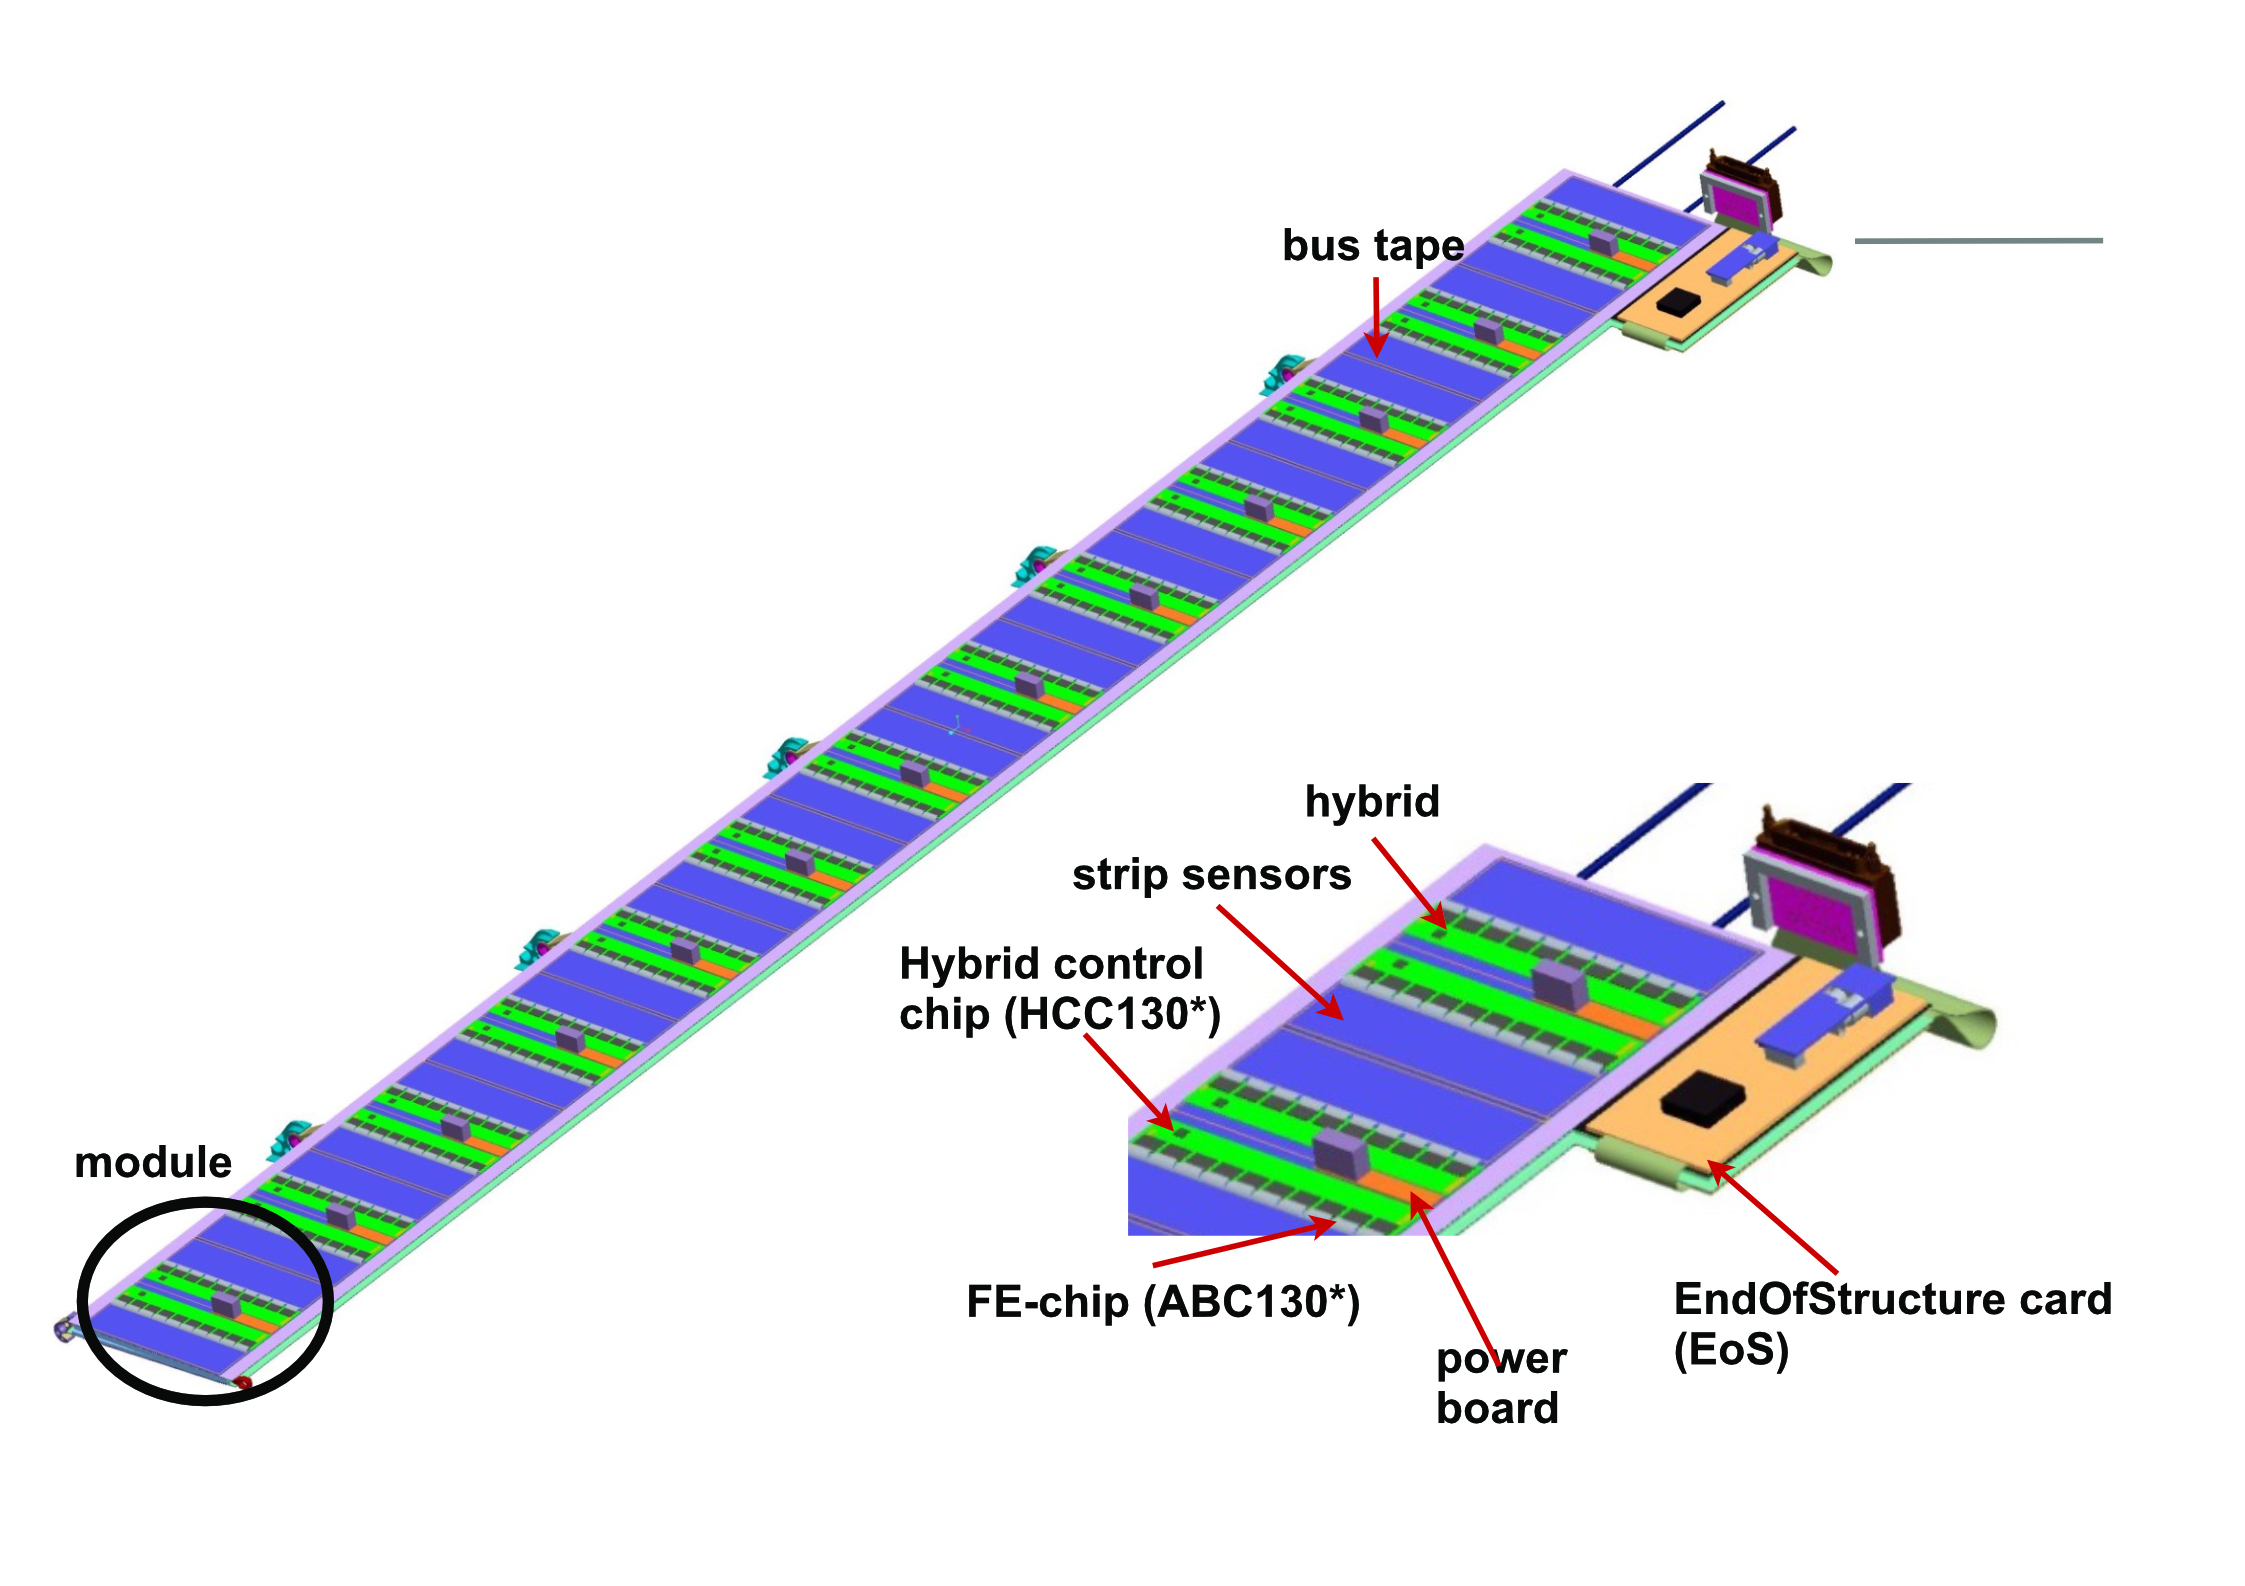
\includegraphics[width=0.8\textwidth]{img/moduleOnStave.jpg}\\	
			\caption{The placement of module (Strips) on the stave \cite[slide 14]{lankfordReviewStrips}.}
		\end{figure}


	\item[Pixel] \hfil \\
		The pixel detector is on of the two main types of the detector. Mounted on staves, the pixels are placed closest to the beam pipe
	\item[Strips] \hfil \\
		The strips are the second type of detectors used inside the ITk structure. The are mounted around the central solenoid (above pixels) and as end caps for the barrel.

	\item[Test] \hfil \\
		Due to the long life expectancy of the ITk and the operation conditions (every part is exposed to radiation during the collision) every component used on the ITk construction has to be properly tested before it can be shipped and assembled into the detector main structure. \cite{vacek}
	

		Test is a generalisation used for the various processes ensuring the quality of all components used for ITk construction. In the context of the Production database, we refer usually refer to all results of such processes as \emph{test}, that are to be recorded and stored inside the database.
		
		The production database has to store all the results for every component for later analysis, if anything breaks in the future.
		
		The database can store various form or types of test results such as scans, chip results, DCS  \footnote{ATLAS \textbf{D}etector \textbf{C}ontrol \textbf{S}ystems \cite{cernDcs}} status or DAQ\footnote{SCTDAQ is a software package which has evolved for testing SCT hybrids and modules at the testbeam, systemtest, PS irradiations, and many institute labs. It runs on a Windows PC. \cite{cernDaq}} information. \cite[p31]{sverma}
		
	\item[Institution] \hfil \\
		Institutions referred in this thesis are 3th party universities, manufactures or various stakeholders of the ITk upgrade project. The are the primary users of the Component database.
\end{description}



\section{The Production database}
\label{sec:theProductionDatabase}
\par The process of building and subsequently maintaining the new inner detector requires a centralised software solution to keep track of all its components. For this purpose the Production database project has been launched at CERN following the plans for the detector upgrade.

\par For the clarification is should be noted that for the purpose of this thesis the term \emph{Production database} implies the entire ICT solution (hosting, applications, client software etc.) and not just relational database as common in the field of IT.

\par The two main functions of the ITk production database can be generalized to data storage (recording items) and data access (report and anylises). These two main groups of use cases are explored in the sections \ref{sec:currentDatabaseStatus} and \ref{sec:notImplemented} of this thesis.


\subsection{Database users}
\par According to Igor Šverma, three users for the component database have been identified so far \cite[page 22]{sverma}. In this context, the term user implies the user group instead of the actual physical user. These groups are:

\begin{description}
	\item[Automated systems] with the rights to write in the database (scans, measurements etc.),
	\item[Atlas ID Community] with the right to read and upload tests, items, assemblies and shipments,
	\item[Manufactures] with the right to upload files to for items.
\end{description}


\par Steve McMahon expands this subject further more in his presentation given on the Prague workshop in June 2015 \cite{databasePresentation} by stating following groups as the basic database users:

\begin{itemize}
	\item testing departments on universities,
	\item manufacturing departments on universities,
	\item contact persons in the factories,
	\item industrial partners (Manufacturers).
\end{itemize}

\par The McMahon's specifications shows, that more detailed privilege could be implemented for the group that Šverma generalises as a Atlas ID Community to ensure the consistency of the database content.

\par The question of Automatic system uploads remains unsolved in the Šverma's thesis and it is expanded in section \ref{sec:notImplemented}.



\section{Current database status}
\label{sec:currentDatabaseStatus}

\par At this moment, the Component Database is in the phase of the development, although it's design is missing some important items, which are explored in section \ref{sec:notImplemented}. The three main components of the database have been prepared in the previous years:

\begin{itemize}
	\item MySQL database,
	\item Java applets (uploaders),
	\item Perl web application.
\end{itemize}


\par The relation between these parts is shown on the figure \ref{fig:currentDatabaseStatus}.

	
\begin{figure}[!ht]
	\centering
	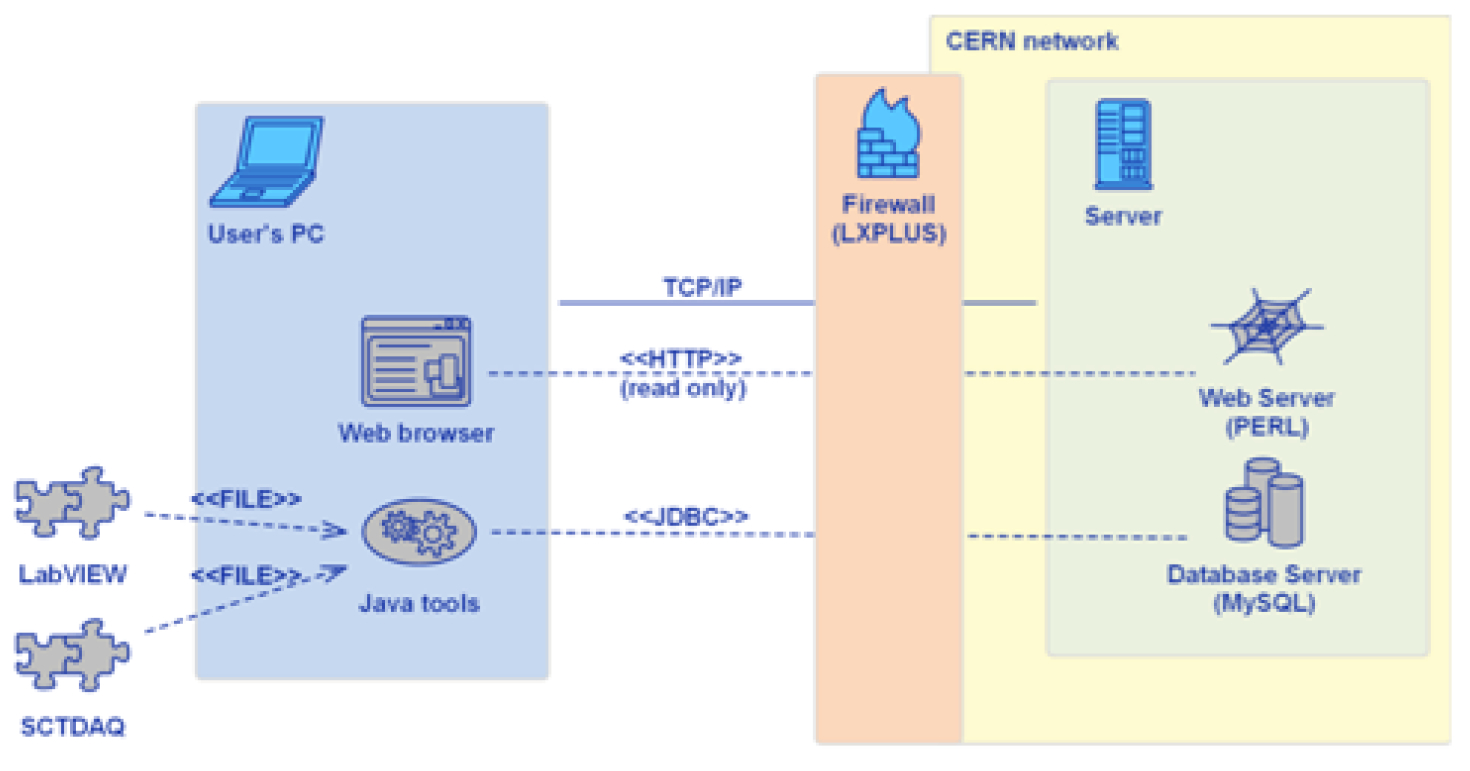
\includegraphics[width=0.8\textwidth]{img/itkCurrentStatus.jpg}\\	
	\caption{The current Component database \cite[slide 4]{presCurrentDatabaseStatus}.}
	\label{fig:currentDatabaseStatus}
\end{figure}


\par The database is currently running on the dedicated Linux server hosted at CERN network with the replication server established in Prague \cite[slide 5]{presCurrentDatabaseStatus}. The new production server is being installed at the Institutes of Physics of the Czech Academy of Sciences \cite[slide 10]{presCurrentDatabaseStatus} which should serve as the primary database server in the future.


\subsection{Java applets}
\label{sec:javaUploaders}
\par Alternatively referred to as  \emph{Java uploaders}, these are the sets of scripts written in Java language by the ATLAS community\footnote{Dave Robinson, Thomas Kluge, Carlos Garcia-Argos} which are intended to be used as the primary way to interact with the Production database. The work on uploaders began in 2008\footnote{Based on class comments inside the source codes}. The applets are worked by console commands and they are interacting with the MySQL server directly using JDBC\footnote{\textbf{J}ava \textbf{D}ata\textbf{B}ase \textbf{C}onnectivity} connection.

\par Java uploaders lack any proper documentation (both in-code or external) and they do contain all the business logic of the component database (MySQL database servers only as the storage), most of which is contained in one file, that serves as the Model class, called \emph{UMySql.java}.

\par From the brief study of the source codes of Java uploaders, they do lack some patterns that should be common standard in the field, namely:

\begin{description}
	\item [Documentation] written documentation of the functionality (in prose) to explain the basics to uninitiated developer,
	\item [In code comments] written inline comments explaining the execution of code, which are especially helpful in longer classes.
	\item [SQL transactions] The MySQL operations are executed sequentially and are not wrapped in the SQL transaction. If anything occurs during the application run (e.g. connectivity loss or database error), no rollback is possible and the data consistency in the database could be compromised.
	\item [Prepared statements] The MySQL queries lack proper validation and could be used to compromise database content using the SQL injection. 
	\item [Unit test] that are designed to test individual methods. Although we can presume that every method was manually tested during the development, any change to the code threatens to compromise the functionality, since thorough manual testing is required upon every change.
	\item [Refactoring] that could help to clean the code structure. With most of the model layer in one file, this could simplify the in-code navigation for the developer.
\end{description}

\paragraph{Despite these missing patterns, the Java uploaders do the job they were designed for.} However based on my existing knowledge, I would hesitate to call them the optimal and longterm sustainable solution, since they provide room for human and system errors and the entry threshold for new developers is extremely high, mainly due to it's lack of proper documentation and automated tests.


\subsection{MySQL database (Data storage)}
\par The Component database stores the data about the ITk inside the MySQL database, composed of 32 relation tables. The table \ref{tab:mysqlTables} lists all current SQL tables as the summary from more elaborate description in \cite[pages 29-35]{sverma} and \cite[page 58]{sverma}. The complete schema (split into 3 parts for better readability) of the current MySQL database created in \emph{MySQL Workbench} is in the appendix~\ref{app:mysqlSchema}.

\par At this moment, the only way for the database users to insert or update database records is to use the prepared Java uploaders.


\begin{longtable}{|p{4cm}|p{10cm}|}
	\caption{List of current MySQL tables in the database\label{tab:mysqlTables}}
	\\
	
		\multicolumn{2}{l}{\textbf{Test related tables}} \\ \hline
		tests & Table to store test information \\ \hline
		chipresults & Store chip results, one entry per hybrid/chip/test parameter.\\ \hline
		comments & Table that stores comments for tests\\ \hline
		chipstatus & Stores the saves chip status as a String \\ \hline
		daqinfo & Stores DAQ information\\ \hline
		dcsdata & Stores DCS status\\ \hline
		scans & Contains test scan information\\ \hline
		defects & If any defect occurs during the test, it is stored here\\ \hline
		defect\_descr & In this table there are definitions of defects.\\ \hline
		raw\_data & Designed to store optional raw data for the test\\ \hline
		asicresults & \emph{todo} \\ \hline  %ToDO ??dafuq
		genericdata & The unused table for test data\\ \hline
				
		\multicolumn{2}{l}{\textbf{Item related tables}} \\ \hline
		items & This table is the main table to store items in the database. \\ \hline
		locations &  includes id of location from table 'locations', and column 'ctype' is there as a relation with the table 'ctypes'.\\ \hline
		persons & This table saves names of all persons.\\ \hline
		ctypes & Table where types of components are defined.\\ \hline
		ctype\_mfrs &  Identifies which manufacturers are able to create components (of a related type)\\ \hline
		assemblies & information and records the way items are assembled together\\ \hline
		assm\_descr & Contains the description of the assembly\\ \hline
		manufacturers & Holds information about manufacturers\\ \hline
		batches & Stores the information about items that are supplied in batches \\ \hline
		btype\_mfrs & Identifies which manufacturers are able to create batch items (of a related type)\\ \hline
		btypes & Defines the possible types of batches\\ \hline

		\multicolumn{2}{l}{\textbf{Data storage related tables}} \\ \hline
		generic\_categories & Stores the categories for the generic data entries\\ \hline
		genericdates & Stores generic dat of MySQL \emph{date} datetype\\ \hline
		genericfiles & Stores generic dat of MySQL \emph{longblob} datetype\\ \hline
		genericfloats & Stores generic dat of MySQL \emph{float} datetype\\ \hline
		genericints & Stores generic dat of MySQL \emph{int(11)} datetype\\ \hline
		genericstrings & Stores generic dat of MySQL \emph{varchar(80)} datetype \\ \hline
		


		\multicolumn{2}{l}{\textbf{Configuration related tables}} \\ \hline
		configuration & This table supplements the missing configuration file (since there is no application above SQL) and contains the current version of the database \\ \hline
		testnames &  Stores names of all recognised tests \\ \hline
		variables & The table is intended for saving variable labels. \\ \hline
		
\end{longtable}


%ToDo missing indexes over more columns


\subsection{Perl web application (Data access)}

%ToDo Využívání dat
\par Reports and research, popsání stávajícího rozhraní v Perlu

\par The last finished part of the Component database is the Perl web application, written by Dave Robinson. It simple design allow user (without any autorisation) to access the basic statistics about the database content and to list any of the recorded results item or the test result based on it's serial number.

\begin{figure}[!ht]
	\centering
	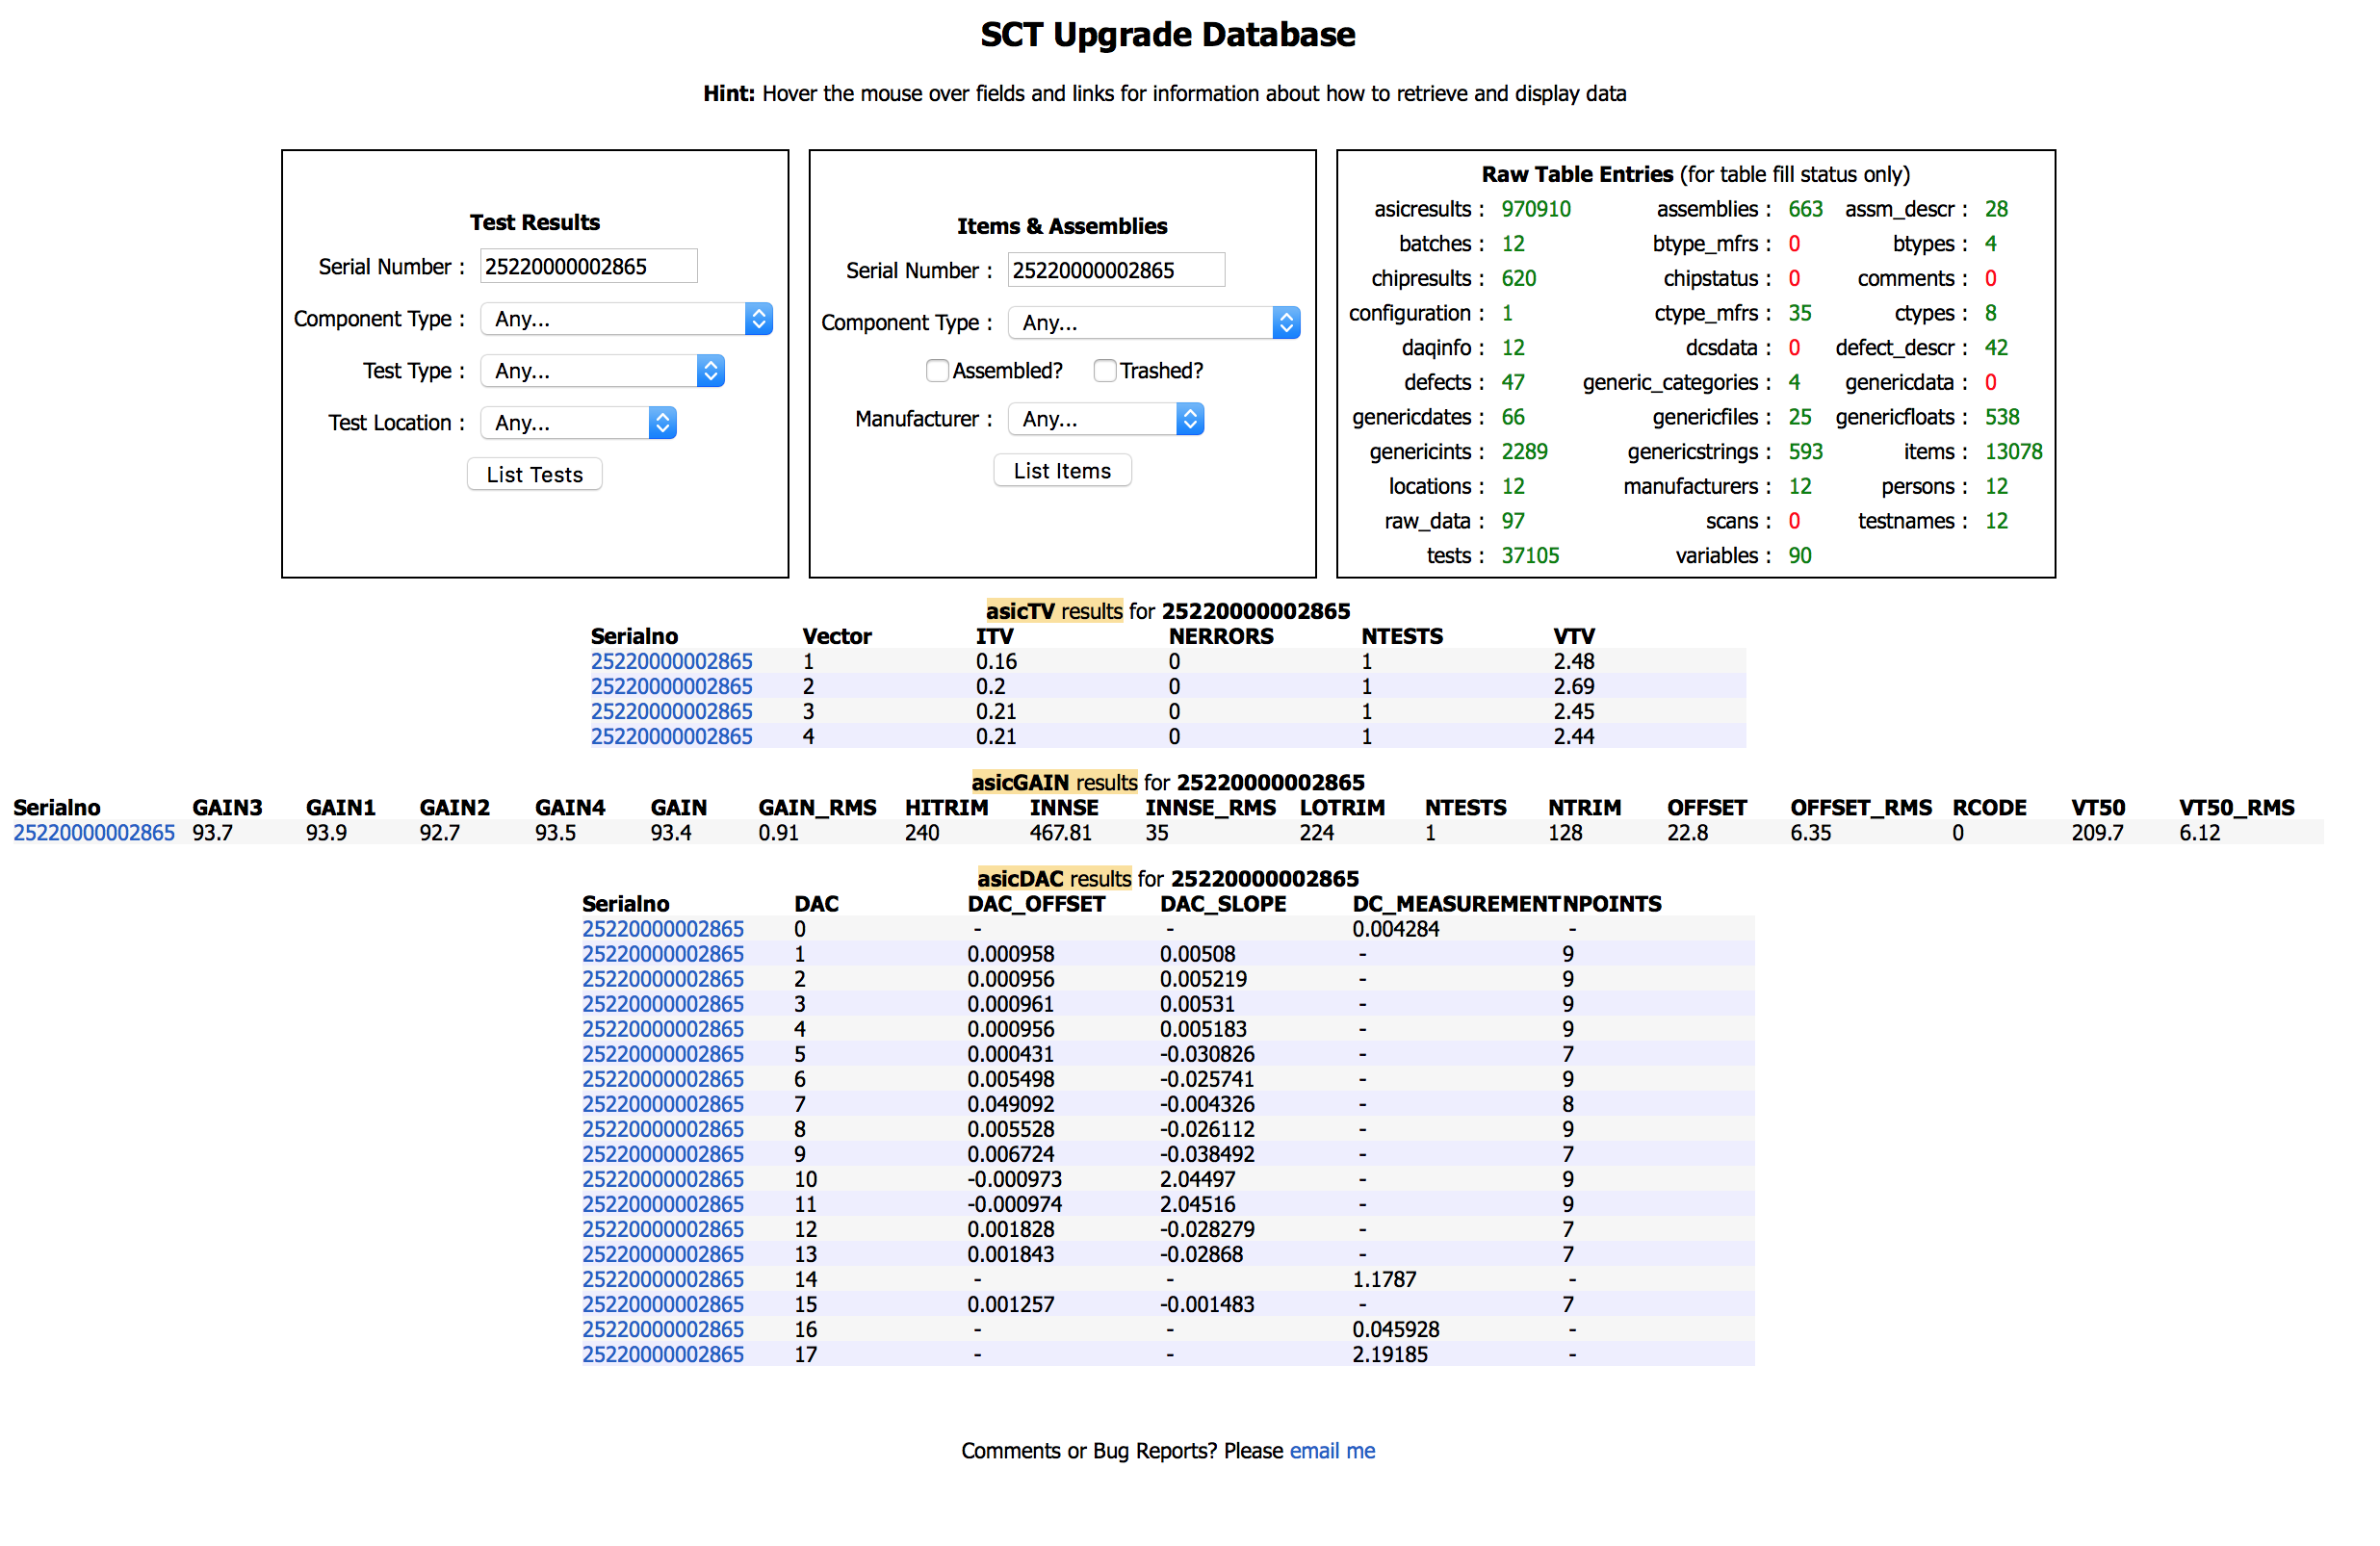
\includegraphics[width=0.9\textwidth]{img/perlWebApp2.png}\\	
	\caption{Perl web app: item detail listed by his serial number}
\end{figure}

\par In the similar way as the Java uploaders, the Perl script has some issues in it's design that prevent any easy alternations of it's functionality. The Perl web interface is purely utilitarian, it lacks the MVC design (the HTML template is directly incorporated into the Perl code and the controllers are nonexistent) and have other issues are similar to the Java uploaders described in section~\ref{sec:javaUploaders}, like the lack of prepared statements or documentation of any kind.

\par Given this limitations, the Perl app is not suitable for any future development and, after proper analysis of the user group's requirements the same functionality will be replicated in the new Web application, but using the implemented API layer in the chapter~\ref{chap:webApp}.

\par The perl scripts are used for accessing the database content in the form of the simple web interface.


\section{Not implemented parts and future development}
\label{sec:notImplemented}
\par As the production database is currently still being developed, it is missing several key parts for it’s proper functionality:

%ToDo Zdroje elaborovat
\begin{itemize}
\item The storage of the pixel detector part
\item Store information that assembly is composed of multiple assemblies. The assemblies should be interconnected to simulate the tree-like structure of the detector construction. 
\item The batches are excluded from the tree-like structure of the inner detector construction
\item Details of performance quality assurance process by testing multiple stages of the component assembly
\item Store test results	 in relation to item not the facility that conducted the test
\item Shipments tracking (what was shipped (including item batches and multiple items per shipment), from where, to where, dates and persons involved)
\item Reporting (Enter item SN and get all details, files and position in the structure)
\item Reporting QA (show tests results, what parts are failing, what tests)
\item Upload more results/files using the batch upload
\item Upload files (tests \& descriptions) from proprietary software like labview/stcdaq/probestation code
\item Registration and assignment of serial numbers to hybrids, on receipt of the hybrid panel by the institute
\item User autorization/authentization, solution for data security
\item Use CERN 14 digits convention, but some parts have serials outside the range
\item The support of shipment tracking on the database level
\item The selection and implementation of a suitable hosting solution
\item Proper versioning of the source codes in a public repository
\item The question of automated systems
\end{itemize}

\paragraph{Several of these changes are blockers for the development of the API,} since they could significantly change the business logic of the ITk database upon which the API should be build. These blockers have to be removed %ToDo

\section{Database usage and limits}
\label{sec:databaseUsage}
%ToDo Tohle přepsat
\par First part of this thesis considers itself with the gathering of necessary materials for proper development. This includes mainly the detailed description of the current database usage (internal processes) and, if possible, the usage data of the current ITk database. Such data are going to be used for proper selection of programming languages and other technologies for the REST API layer and web fronted implementation. If they will be kept up to date, the acquired data will also provide a highly valuable assets for the future database development in the upcoming years.


\subsection{Old database data}
\par The old STK database, 
%Todo Ozdrojovat

The table~\ref{tab:sctUsage} shows the usage statistics from the old SCT component database.

\begin {table}[H]
\begin{center}
	\caption{The SCT database statistics~\cite[slide 4]{cambridgeSctPresentation}}
	\label{tab:sctUsage} 
	
    \begin{tabular}{ | l | l |}
    \hline
    Item & Amount \\ \hline
	Database size & 7 GB\\ \hline
	Num. of rows in one table & approx. 38 000 000\\ \hline
	Inserted item types & 220 \\ \hline
	Inserted items & 349 686\\ \hline
	Inserted shipments & 4 506\\ \hline
	Inserted num. of shipped items & 632 508 \\ \hline
	Inserted types of test & 52\\ \hline
	Inserted test results & 1 122 196\\ \hline
	Inserted assembly test definitions & 4 571\\ \hline
	Inserted assemblies & 130 210\\ \hline

    \end{tabular}

\end{center}
\end{table}
    
\subsection{Usage predictions}
- 20 000 stip modules, 10 000 pixel modules
- currently ~24 countries on the candidate lists, more institutions per country, most of them working with both strips and pixels
- Max. hundreds per institution
- Multiple types of users in every institution
— University - testing department
— University - manufacturing department
— Contact person in the factory
— Manufacturers

%ToDo My usage prediction, nějaký grafík
Just by the number of modules we can estimate

\section{Summary}
\par As we can see, the Component database is in still in the early stage of it's lifecycle. Although a~large effort has been put to some crucial parts like test storage or parameter generalisation and the SQL schema is nearly in its final iteration,  the overall design still lacks some key features that have to be resolved and implemented before the phase of API design can commence.

\par In the next chapter, I will describe the goal of the proposed API layer, explore current implementation of the record insertion and propose some improvements that the API can bring into the component database system. 

\par I will try to resolve the missing functionality at the beginning of the design phase in the chapter~\ref{chap:apiArchitecture}.


\chapter{API goal}
\label{chap:apiGoal}
\par The main goal of this thesis is to propose and implement a functional, usable and deployable REST API application for the Production database. The REST API should replace the direct access to MySQL database used by Java applets.

\par While the direct database access provides easy and comfortable solution for a single developer, it is not suitable for the software solution of requested size and lifespan, as it lacks some advance features that are required:

\begin{itemize}
	\item request tracking with easy to analyse logs
	\item ACL implementation
	\item data consistency assurance (anyone with write access can adjust the table content)
	\item testability in the case that someone has changed the database layout
	\item protection from table deadlocks
	\item query analyse for debugging (although MySQL platform does offer the „Slow query log” it is very difficult to pair the problematic SQL queries to specific time when the server monitoring has encountered some performance issue)
	\item no development environment for new developers
\end{itemize}

With this in mind, the API architecture needs to be devised before the implementation phase to prevent any unwanted results when working with the production database.


\par Based on the facts stated in section~\ref{sec:theProductionDatabase} of the thesis, the main usage of the API should mirror the use cases of the MySQL database and can be divided in the same way as the usage of the component database itself: date selection and date insertion/update.


\par Another possible issue that could occur in the future if the database's lifetime is the performance issue regarding the SQL SELECT queries over multiple items having the generic values.
	
\par From my experience\footnote{Work at Brand New s.r.o., Prague 2014}, trying to emulate the free key:value structure using the generic param/value rows in SQL lead to significant performance issues in the length of the query execution with the number of rows exceeding 1 million rows.

\par The API layer will easily solve this issue by caching the relations as proxy objects and serving those preserialized proxies upon new http request.
	


%ToDo citovat už tady nějaké věci

%ToDO stávající popis architetktury, proč je to blbě
\ref{fig:currentDatabaseStatus}

%ToDO Má představa funkčnosti
\chapter{API architecture}
\label{chap:apiArchitecture}

%ToDo Obrázek navrhované architektury

\begin{itemize}
	\item resolving the missing feature issues
	\item api mockup \& documentation
	\item api application layer
	\item programming language selection
	\item deployment
	\item The full list and descriptions of proposed endpoints and their mockups
\end{itemize}



\par The user has a relation to manufactures table if the user is a registered manufacturer for the ITk.

\par Manufactures can add a component only if they are elegible to manufacture a component of requested type. The check is done using the ctype\_mfrs relation table.

\par To ensure the data consistency, the MySQL views should be prepared.
\chapter{API implementation}
\label{chap:apiImplementation}
\section{Materials}
\par The following part of the thesis is the implementation of the REST API layer and the implementation of a web interface.
	
\par The API Layer provides the data source for all 3th party tools and services, including the web interface and possible handheld applications. Considering the nature of the database content, special care is given to the authorisation and user privileges handling, so no unauthorised user is able to access or change the database content.
\chapter{API tests and ensuring future consistency}
\label{chap:apiTests}
%ToDo Capter API tests
ToDo:
\begin{itemize}
	\item dummy data (e.g. fixtures)
	\item extreme load tests to simulate the peaks in the lifecycle
	\item automated API tests for future developers
	\item code checkers to ensure the code consistency
	\item deprecated application exception for old java uploaders
	\item test enviroment for future developers
\end{itemize}


\par Base on the usage predictions, the example big data needs to be generated to simulate the real working conditions of the production database (fixtures).

\par Direct access to the database should be disabled and only the database user used by the API application should be able to directly interact with the MySQL installation on the production server. In that case, all future requests for new features have to be implemented as an API request first, which in return guarantees that the backward compatibility is checked by automated tests when releasing an updated version.

\par The situation, when somebody in the 3th party institution is not able to get requested information from the web interface because somebody irreversibly changed the data integrity by bypassing the API via the socket connection to the database, has to prevented.


\chapter{Web interface for the API}
\label{chap:webApp}
\par An easy to use web interface, which is using such layer. Using the web interface, users can access the database data in a fast and comfortable way.

\par The web interface is sing the data provided by API layer and provides a simple and easy-to-use access to the database content. The implementation of the API layer includes the proposal for a future user roles implementation and data insertion, which could remove the need of using dedicated javascript for unschooled users.
\par To demonstrate future possibilities of usage on handheld devices, the simple iOS application using the web wrapper and the responsive web interface is created as a part of this thesis.




%ToDo Thesis summary

\chapter{Summary}
\label{chap:summary}
%ToDo Thesis summary
Summarise the thesis Goal, compare the published API and the requirements, add feedback from the ATLAS community to the API and the web interface.

%Seznam použitých zdrojů
\begin{thebibliography}{2}
\label{bibliography}

	\bibitem[Richardson, Amundsen, Ruby 2013]{restapi} L. RICHARDSON, M. AMUNDSEN, S. RUBY: \emph{RESTful Web APIs}. 1st Edition, O’Reilly Media, ISBN 9781449358068 , Kindle Edition, 2013, pp. 406 
   
	\bibitem[Šverma 2015]{sverma} Igor ŠVERMA: \emph{A Component Database Design for the ATLAS Inner Detector at LHC}. Unicorn College s.r.o. 2015, pp. 97  Bachelor’s thesis at Unicorn College at Department  of information  technologies. Supervisor of the Thesis doc. Ing. Václav Vacek, CSc.

	\bibitem[ATLAS ITk website]{atlasitkweb} \emph{Detector description Inner Detector} [online] [quoted 2015-01-02] Available on: <\url{http://www.atlas.ch/inner-detector.html}>

	\bibitem[ATLAS website]{atlasweb} \emph{ATLAS Experiment} [online] [quoted 2015-01-08] Available on: <\url{http://www.atlas.ch/what\_is\_atlas.html}>

	%ToDo tady možná nesedí TDR ISBN
	\bibitem[Atlas TDR 1 1997]{atlas1} ATLAS COLLABORATION: \emph{ATLAS Inner Detector TDR (Technical design report)}, Vol. 1(ISBN 92-9083-102-2) and Vol. 2 (ISBN 92-9083-103-0), CERN/LHCC/97-16, Geneva, 1997, pp. 254
    
	\bibitem[Atlas TDR 2 1997]{atlas2} ATLAS COLLABORATION: \emph{ATLAS Inner Detector TDR(Technical design report), Vol. 2}. Vol. 2 (ISBN 92-9083-103-0), CERN/LHCC/97-16, Geneva, 1997, pp.898
 
	\bibitem[Bie 2015]{apitheory} M. BIEHL: \emph{API Architecture : The Big Picture for Building APIs (API-University Series Book 2)}, ISBN: 150867664X, Kindle Edition, 2015,  pp. 192
	\bibitem[MySQL website]{mysqlweb} \emph{4.2.2 Connecting to the MySQL Server} [online] [quoted 2016-01-04] Available on: <\url{https://dev.mysql.com/doc/refman/5.5/en/connecting.html}>
	
	\bibitem[Robinson 2015]{cambridgeSctPresentation} Dave ROBINSON: \emph{Previous Experience of Databases - The SCT ProducGon Database A (similar) database for ITK} 	[presentation] Prague: ITk Database Workshop, 2015-06-25
	
	\bibitem[McMahon 2015]{databasePresentation} Steve McMAHON: \emph{Production Databases Introduction, requirements, schedule: What, Why, When, Where, Who} 	[presentation] Prague: ITK Database Workshop, 2015-06-25
	
	\bibitem[Gregor,Affolder 2015]{lankfordReviewStrips} Ingrid-Maria GREGOR, Tony AFFOLDER on behalf of the ITK Strip Community: \emph{ITK Strips Status and Plans towards TDR} [presentation] ATLAS Lankford Review, 2015-11-23
	
	\bibitem[Vacek 2015]{vacek} doc. Ing. VACEK, Václav CSc., [ústní sdělení] V Kapslovně 2767/2  Praha, 2015-11-18
	
	\bibitem[Atlas]{atlasExperiment} ATLAS COLLABORATION: \emph{The ATLAS experiment at the CERN Large Hadron Collider}, (ISBN ToDO), pp. 408
	
	\bibitem[GLA website]{glasgowWeb} \emph{ATLAS Semiconductor Tracker (SCT) and Inner Detector (ID)} [online] [quoted 2015-01-08] Available on: <\url{http://www.gla.ac.uk/schools/physics/research/groups/particlephysicsexperiment/researchoverview/detectordevelopment/activities/atlassemiconductortrackersct}>

	\bibitem[CERN Atlas SCT Test website]{cernDaq} \emph{Atlas SCT Test DAQ Online Documentation} [online] [quoted 2015-01-03] Available on: <\url{http://sct-testdaq.home.cern.ch/sct/sctdaq.html}>
	
	\bibitem[CERN Atlas DCS]{cernDcs} \emph{ATLAS  
Detector Control Systems} [online] [quoted 2015-01-03] Available on: <\url{http://atlas.web.cern.ch/Atlas/GROUPS/DAQTRIG/DCS/dcshome.html	}>

	\bibitem[Vacek,Beránek 2015]{presCurrentDatabaseStatus} \emph{ITk Production Database Present Status} [presentation] CERN: ITk Week, 15/09/2015
   
   
\end{thebibliography}

\pagebreak



%Seznam obrázků
\listoffigures
 
%Seznam tabulek
\listoftables

\chapter{Extended summary}
%ToDo Extended summary

\begin{appendices}
	\chapter{MySQL Schema}
	\label{app:mysqlSchema}
	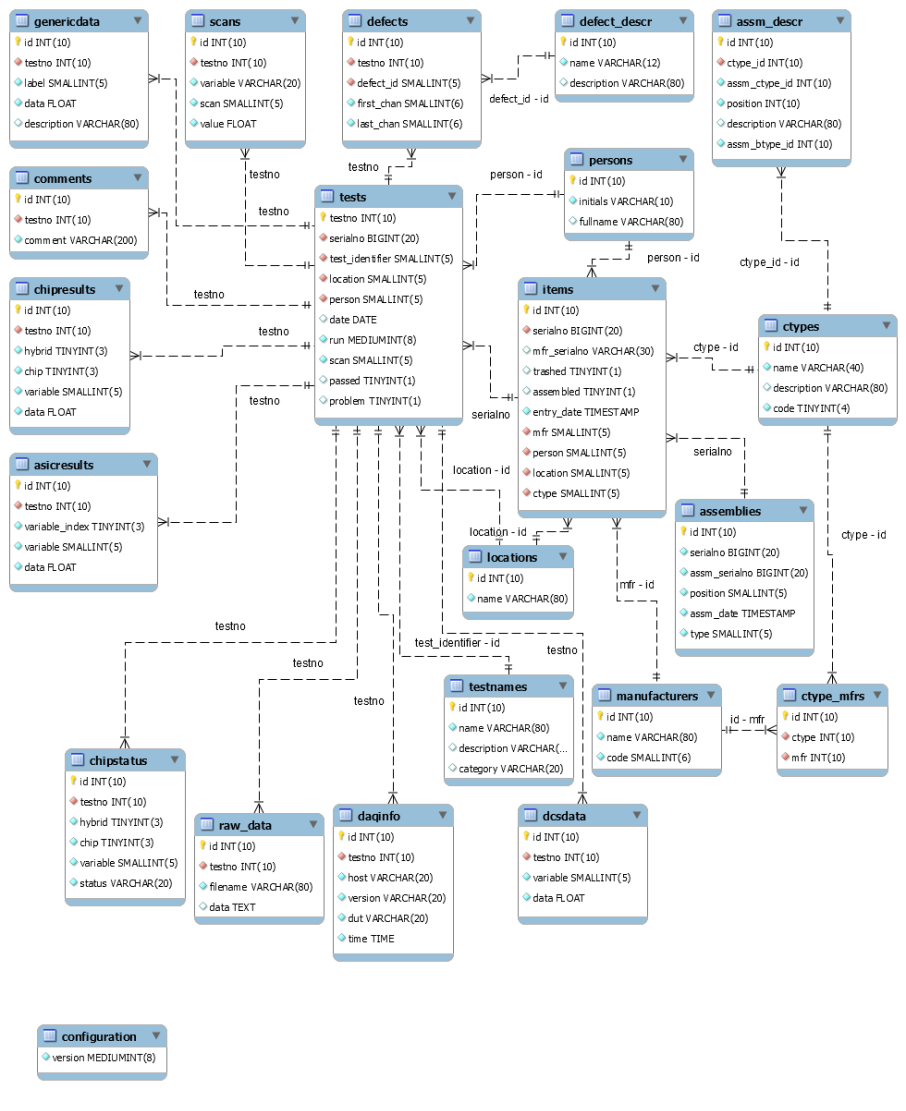
\includegraphics[width=0.9\textwidth]{img/mysql_schema_items.png}\\
	\newpage
	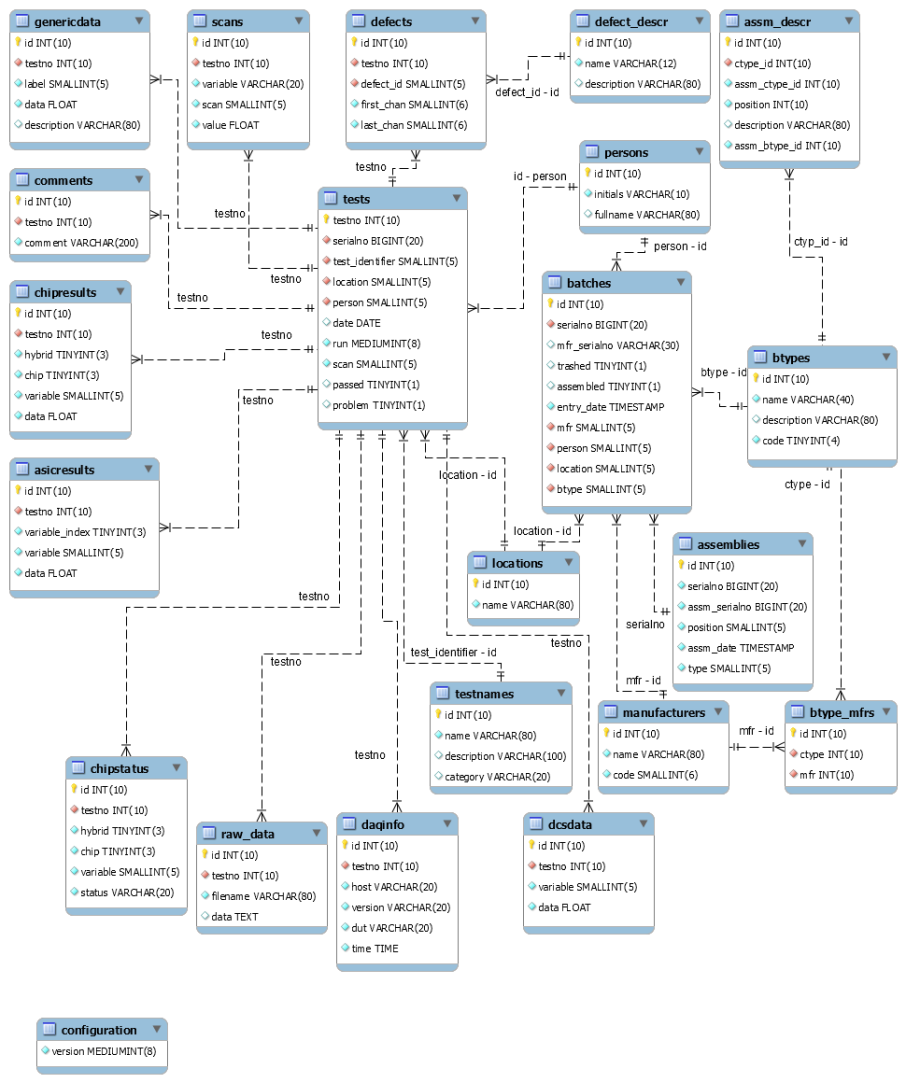
\includegraphics[width=0.9\textwidth]{img/mysql_schema_batches.png}\\
	\newpage
	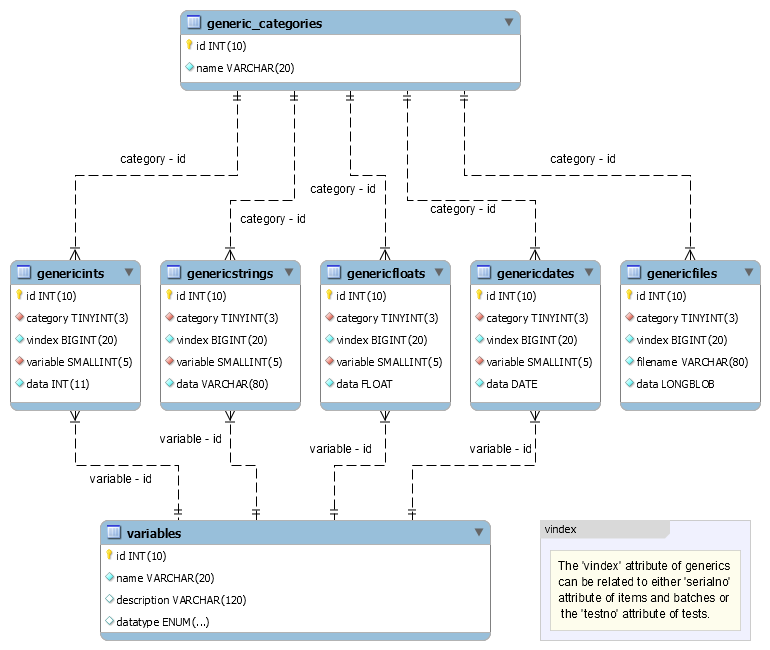
\includegraphics[width=1.0\textwidth]{img/mysql_schema_variables.png}
\end{appendices}


\end{document}